\section{Objetivos}
O presente trabalho tem por objetivo construir um diagrama de equilíbrio
líquido-vapor (ELV) para uma mistura de um polímero (poliisobutileno - PIB) com
um solvente (benzeno). Para isso, será apresentada uma breve discussão dos
modelos e metodologia de cálculo, assim como a teoria aplicada.

\section{Introdução Teórica}


A teoria de \citeonline{Flory1951} e \citeonline{Huggins1942} considera a
energia livre de Gibbs da mistura do polímero puro com o solvente
($\Delta g_{mis}$) em termos de duas contribuições: entalpia de mistura 
($\Delta h_{mis}$) e entropia de mistura ($\Delta s_{mis}$), conforme é
apresentado a seguir:

\begin{equation}\label{eq:gemist}
\Delta g_{mis} = \Delta h_{mis} - T\Delta s_{mis}
\end{equation}
onde $T$ é a temperatura absoluta.

A entropia de mistura é determinada pelas frações volumétricas do solvente
($\phi_1$) e do polímero ($\phi_2$), enquanto a entalpia é determinada pelo
parâmetro adimensional de interação $\chi$, o qual normalmente é referido como parâmetro de interação de
Flory-Huggins, conforme é apresentado nas equações abaixo: 

\begin{equation}\label{eq:entalexc}
\Delta h_{mis} = \chi RT\left( x_1 + mx_2 \right)\phi_1\phi_2
\end{equation}

\begin{equation}\label{eq:entroexc}
\Delta s_{mis} = -R\left( x_1\ln\phi_1 + x_2\ln\phi_2 \right)
\end{equation}

De acordo com \citeonline{Koretsky2013}, a energia de Gibbs em
excesso ($g^E$) é expressa através da diferença entre $\Delta g_{mis}$ e sua
condição ideal, como mostrado abaixo:

\begin{equation}\label{eq:geexc1}
g^E = \Delta g_{mis} - \Delta g_{mis}^{ideal}
\end{equation}
onde:

\begin{equation}
\Delta g_{mis}^{ideal} = RT\sum_ix_i\ln x_i
\end{equation}

Substituindo na \autoref{eq:geexc1}, obtem-se:

\begin{equation}
g^E = \Delta g_{mis} - RT\sum_ix_i\ln x_i
\end{equation}

Através da definição de $\Delta g_{mis}$ e considerando um sistema binário,
tem-se:

\begin{equation}\label{eq:geexc2}
g^E = \Delta h^{mist} - T\Delta s^{mist} - RT\left( x_1\ln x_1 + x_2\ln x_2
\right)
\end{equation}

Substituindo as Equações \ref{eq:entalexc} e \ref{eq:entroexc} na
\autoref{eq:geexc2} e fazendo-se as devidas simplificações, obtem-se uma
expressão para a energia de Gibbs em excesso em função das frações molares
($x_i$) e volumétricas ($\phi_i$), como é apresentado abaixo:

\begin{equation}\label{eq:geRT}
\frac{g^E}{RT} = \chi\left(x_1 + mx_2\right)\phi_1\phi_2 +
\left[x_1\ln\frac{\phi_1}{x_1} + x_2\ln\frac{\phi_2}{x_2}\right]
\end{equation}
onde $x_1$ e $x_2$ são as frações molares do solvente e do polímero,
respectivamente; $\phi_1$ e $\phi_2$ são, respectivamente, as frações
volumétricas do solvente e polímero, as quais são obtidas através das
seguintes equações:

\begin{equation}\label{eq:fracvap}
\phi_1 = \frac{n_1}{n_1 + mn_2}
\end{equation}

\begin{equation}
\phi_2 = \frac{mn_2}{n_1 + mn_2} = 1 - \phi_1
\end{equation}
onde $m$ é o número de repitições da unidade de monômero contida na cadeia
polimérica e pode ser obtida através da razão entre massa molar do polímero
($M_{wp}$) pela do monômero ($M_{wm}$), como é apresentado a seguir:

\begin{equation}
m = \frac{M_{wp}}{M_{wm}}
\end{equation}

 Aplicando-se a definição de uma
propriedade parcial molar para a \autoref{eq:geRT}, ou seja, realizando-se a
diferenciação com relação ao número de mols do solvente, obtem-se
a seguinte expressão para o coeficiente de atividade para tal
componente da mistura ($\gamma_1$):


\begin{equation}\label{eq:gamma1}
\ln\gamma_1 = \ln\frac{\phi_1}{x_1} + \phi_2\left( 1 - \frac{1}{m} \right) +
\chi\phi_2^2
\end{equation}

De uma maneira análoga ao que foi feito para a obtenção da \autoref{eq:gamma1},
chega-se na seguinte expressão do coeficiente de atividade para o polímero
($\gamma_2$):

\begin{equation}
\ln\gamma_2 = \ln\frac{\phi_2}{x_2} - \phi_1\left( m - 1 \right) +
m\chi\phi_1^2
\end{equation}

Conforme é apresentado por \citeonline{Tadros2013}, o parâmetro de interação de
Flory-Huggins ($\chi$) fornece a medida da interação das cadeias poliméricas com as moléculas de solvente e, também, as interações
polímero-polímero. 

Quando $\chi$ assume valor igual a $1/2$, o polímero se comporta
como uma mistura ideal com o solvente e, nessa condição, é denotado por Flory
como ponto $\theta$. Desse modo, o polímero não sofre nenhum tipo de repulsão ou
atração. Para valores de $\chi$ inferiores a $1/2$, a mistura
se comporta como não ideal, apresentando desvios positivos (repulsão). 
Em contrapartida, para $\chi$ superior a $1/2$, ocorrem desvios negativos
(atração). Nessas condições, pode haver a precipitação do polímero.

Conforme é apresentado por \citeonline{Lindvig2002}, a relação entre o parâmetro
de interação de Flory-Huggins e o parâmetro de solubilidade é apresentada
através da seguinte expressão:

\begin{equation}
\chi = \frac{v_1}{RT}\left( \delta_1 - \delta_2 \right)^2
\end{equation}

Os parâmetros
de solubilidade dos componentes puros ($\delta_1$ e $\delta_2$), conforme
\citeonline{Kwak1986}, podem ser obtidos a partir da energia interna de
vaporização de cada componente puro $i$ ($\Delta u_i^v$), como um líquido saturado na temperatura do sistema
(\autoref{eq:deltai}):

\begin{equation}\label{eq:deltai}
\delta_i = \left ( \frac{\Delta u_i^V}{\nu_i^L} \right )^{\frac{1}{2}}
\end{equation}

O termo entre parânteses da \autoref{eq:deltai} é denominado de densidade de energia
coesiva e o parâmetro de solubilidade para misturas multicomponentes é mostrada
na \autoref{eq:delta}:

\begin{equation}\label{eq:delta}
\delta = \sum_i\sum_j\phi_i\phi_j\delta_{ij}^2
\end{equation}
onde

\begin{equation}\label{eq:deltaij}
\delta_{ij}^2 = \delta_i\delta_j
\end{equation}



\section{Metodologia}

Para a realização do estudo do equilíbrio líquido-vapor da mistura
polímero - solvente contendo benzeno e poliisobutileno (PIB) utilizaram-se 
os dados experimentais (retirados do material fornecido em aula) apresentados na
\autoref{tab:dexp2}. As propriedades, necessárias para os cálculos, das duas
substâncias envolvidas no estudo estão mostradas na \autoref{tab:dexp1}.

\begin{table}[htb]
\renewcommand{\arraystretch}{1.3}
\centering
\caption{Dados experimentais de ELV da mistura polímero-solvente benzeno(1) /
PIB(2) a 312,75 K.}
\begin{tabular}{S[table-format=2.2,round-mode=places,round-precision=2]
S[table-format=1.4,round-mode=places,round-precision=4]}
\toprule
{$w_1$ (\%)}	&	{P (bar)}	\\
\midrule

4,37	&	0,0715	\\
6,33	&	0,0971	\\
9,45	&	0,1236	\\
15,16	&	0,1681	\\
18,42	&	0,1818	\\
25,37	&	0,2095	\\
29,71	&	0,2182	\\
32,12	&	0,2207	\\
37,30	&	0,2267	\\
\bottomrule
\end{tabular}
\label{tab:dexp2} 
\end{table} 

\begin{table}[htb]
\renewcommand{\arraystretch}{1.3}
\caption{Propriedades dos componentes da mistura polímero-solvente benzeno(1) /
PIB(2)}
\sisetup{table-format=2.2,round-mode=places,round-precision=2}
\footnotesize
\center
\begin{tabular}{lrlr}
\toprule
\multicolumn{2}{c}{Benzeno (1)}	&	\multicolumn{2}{c}{PIB (2)}		\\
\cmidrule(lr{.5em}){1-2} \cmidrule(lr{.5em}){3-4}
{$M_{w1}\rm{ (g/mol)}$} 	&	{$78$}	&	{$M_{wp}\rm{ (g/mol)}$}	&	{$40000$}	\\
{$v_1\rm{ (cm^3/mol)}$}	&	{$88,26$}	&	{$M_{wm} \rm{ (g/mol)}$}	&	{$104$}	\\
{$P_1^{sat}\rm{ (bar)}$}	&	{$0,2392$}	&	{$v_m \rm{ (cm^3/mol)}$}	&	{$131,9$}	\\

\bottomrule
\multicolumn{4}{c}{Obs.: Dados retirados do material fornecido em aula}
\end{tabular}
\label{tab:dexp1}
\end{table}

Apenas para nível de comparação, a \autoref{tab:prop1} mostra alguns valores
experimentais de $\chi$ para a mistura benzeno/PIB para diferentes composições e
faixas de temperaturas.

\clearpage

\begin{table}[htb]
\centering
\renewcommand{\arraystretch}{1.3}
\caption{Valores experimentais de $\chi$ em função da temperatura e da fração
volumétrica do polímero ($\phi_2$) encontrados na literatura}
\begin{tabular}{lcc}
\toprule
{Temperatura ($^\circ$C)} & {Fração Volumétrica ($\phi_2$)} & {$\chi$}		\\
\midrule
{$	10			$}	&	{$	0,4$	a	$0,8$}	&	{$	0,670$	a	$0,920$	}	\\
{$	25			$}	&	{$	0,0$	a	$1,0$}	&	{$	0,498$	a	$1,060$	}	\\
{$	25			$}	&	{$	1,0$	 		}	&	{$	0,880$	a	$0,610$	}	\\
{$	27$	a	$65	$}	&	{$	0,6$	a $1,0$	}	&	{$	0,730$	a	$1,070$	}	\\
{$	30			$}	&	{$	0,0$			}	&	{$	0,495$				}	\\
{$	40			$}	&	{$	0,6$	a $0,8$	}	&	{$	0,700$	a	$0,800$	}	\\
{$	50			$}	&	{$	0,0$	a $0,2$	}	&	{$	0,485$	a	$0,583$	}	\\
{$	100			$}	&	{$	1,0$			}	&	{$	0,700$				}	\\
{$	37$	a	$200$}	&	{$	1,0$			}	&	{$	1,180$	a	$0,700$	}	\\

\bottomrule
\multicolumn{3}{c}{Fonte:\citeonline{Orwoll2007}}
\end{tabular}
\label{tab:prop1}
\end{table}

Para os cálculos de equilíbrio, utilizou-se o modelo da Lei de Raoult
Modificada, considerando a fase vapor como sendo um gás ideal. O coeficiente de
atividade foi calculado através do modelo de Flrory-Huggins, explanado na seção
anterior.

\begin{equation}
\hat{f_1}^l = \hat{f_1}^v
\end{equation}

\begin{equation}
\gamma_1x_1P_1^{sat} = Py_1
\end{equation}

Como o solvente apresenta-se na forma pura na fase vapor, ou seja, sua fração
molar ($y_1$) é igual a 1,0, tem-se:

\begin{equation}
\gamma_1x_1P_1^{sat} = P
\end{equation}

Como os dados de composição foram apresentados em base mássica, foi necessário
convertê-los em base molar para fazer-se o uso do modelo. A seguir está mostrada
a relação entre as frações mássicas e molares:

\begin{equation}
x_1
=\frac{\displaystyle
\frac{w_1}{M_{w1}}}{\displaystyle\frac{w_1}{M_{w1}}+\frac{w_2}{M_{wp}}}
\end{equation}

A partir disso, é possível reescrever a \autoref{eq:fracvap} em função das
frações mássicas e volumes molares, como é apresentado a seguir:

\begin{equation}
\phi_1 =
\frac{\displaystyle\frac{w_1}{M_{w1}}v_1}{\displaystyle\frac{w_1}{M_{w1}}v_1+\displaystyle\frac{w_2}{M_{wp}}mv_m}
\end{equation}

Os códigos de programação foram implementados em
liguagem $Java$ utilizando o ambiente do Eclipse Mars 2 Release (4.5.2)


\section{Resultados}

\subsection{Sensibilidade do modelo aos valores de $\chi$ }
Nessa seção buscou-se ententer o comportamento do modelo frente a diferentes
valroes de $\chi$. A \autoref{tab:allsets} apresenta as configurações utilizadas
para cada cálculo e utilizou-se $0,50$ como valor inicial de $\chi$ (mistura
ideal) até o valor máximo de $1,50$, com passo de $0,10$.

\begin{table}[htb]
\centering
\renewcommand{\arraystretch}{1.3}
\caption{Valores dos erros médios (absoluto e relativo) para diferentes valores
do parâmetro de interação polímero-solvente ($\chi$)}
\begin{tabular}{S[table-format=3.0,round-mode=places,round-precision=0]
S[table-format=2.0,round-mode=places,round-precision=0]
S[table-format=1.2,round-mode=places,round-precision=2]
S[table-format=1.2,round-mode=places,round-precision=2]}
\toprule
{Valores de}& {Quantidade de} & \multirow{2}{*}{$\chi_{min}$} &
\multirow{2}{*}{$\chi_{max}$}\\
{$w_1$ gerados}& {$\chi$ testados} & &\\
\midrule
100&11&0.5&1.5\\
\bottomrule
\end{tabular}
\label{tab:allsets}
\end{table}

Foram testados, posteriormente, valores de $\chi$ inferiores a $0,50$ e
superiores a $1,50$, porém os resultados apresentaram-se com desvios maiores
com relação aqueles avaliados. Conforme o apresentado na
\autoref{tab:prop1}, praticamente todos os valores de $\chi$ para a mistura em
questão apresentam-se dentro da faixa avaliada.

A \autoref{tab:allresult} apresenta os valores médios dos erros absoluto e
relativo para todos os valores de $\chi$ avaliados. Observa-se que os menores erros
médios ocorrem quando $\chi$ é igual a $1,00$. A \autoref{fig:trab4ki} mostra os
comportamentos do modelo na predição do equilíbrio, frente aos diferentes
valores de $\chi$, comparados com os dados experimentais. Os valores pontuais de
erro absoluto e relativo encontram-se no Apêndice A.

\clearpage

\begin{table}
\centering
\renewcommand{\arraystretch}{1.3}
\caption{Valores dos erros médios (absoluto e relativo) para diferentes valores
do parâmetro de interação polímero-solvente ($\chi$)}
\begin{tabular}{cS[table-format=1.4,round-mode=places,round-precision=4]S[table-format=2.2,round-mode=places,round-precision=2]}
\toprule
& {Erro Médio} & {Erro Médio} 	\\
& {Absoluto} & {Relativo (\%)}	 \\
\midrule 
{$\chi = 0,50$} & 0.0431 & 29.06 \\
{$\chi = 0,60$} & 0.0352 & 24.26 \\
{$\chi = 0,70$} & 0.0268 & 19.11 \\
{$\chi = 0,80$} & 0.0179 & 13.58 \\
{$\chi = 0,90$} & 0.0105 & 8.61  \\
{$\chi = 1,00$} & 0.0093 & 6.38  \\
{$\chi = 1,10$} & 0.0147 & 7.81  \\
{$\chi = 1,20$} & 0.0244 & 12.88 \\
{$\chi = 1,30$} & 0.0368 & 20.77 \\
{$\chi = 1,40$} & 0.0501 & 29.24 \\
{$\chi = 1,50$} & 0.0643 & 38.34 \\
\bottomrule
\end{tabular}
\label{tab:allresult}
\end{table}

\begin{figure}
\centering
{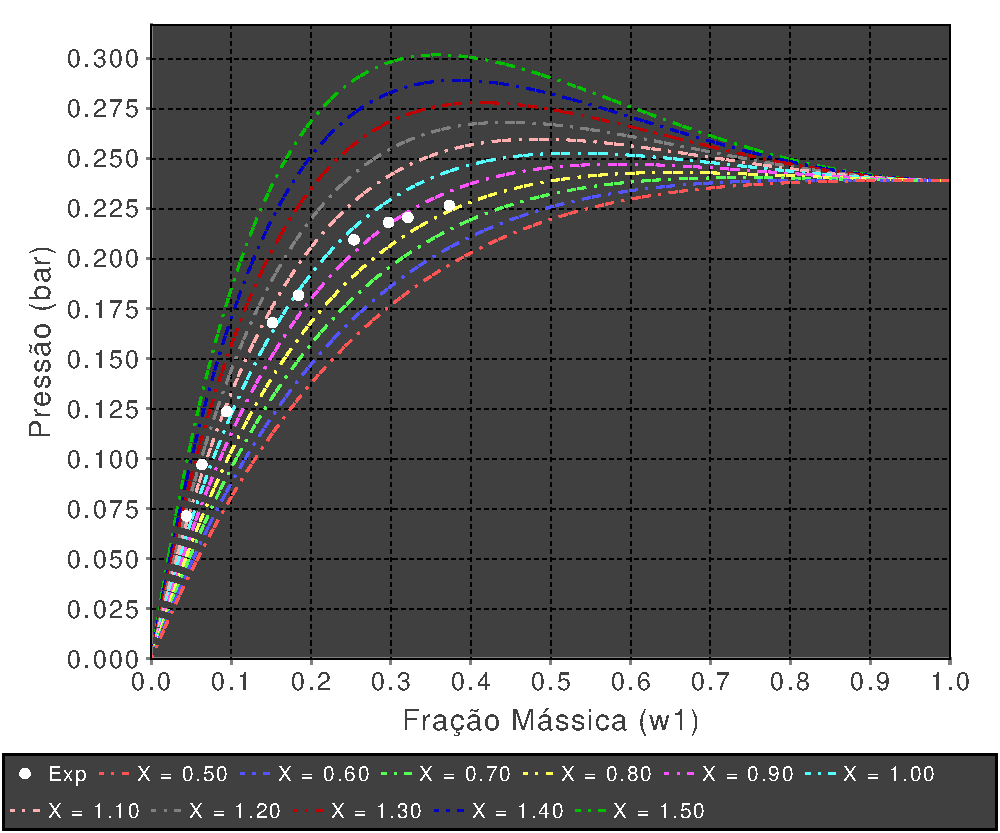
\includegraphics[width=0.8\textwidth]{img/Trab4Ki.pdf}} 
\caption{Curvas $P-w_1$ para diferentes valores de $\chi$}
\label{fig:trab4ki}
\end{figure}

\clearpage

\subsection{Otimização}
Otimização de processos pode ser matematicamente descrita como uma busca por um
máximo ou mínimo de uma função objetivo. Assim, neste trabalho, a função objetivo escolhida 
foi o somatório do diferencial da pressão calculada a partir dos parâmetros
$\chi$ com a pressão experimental. Entretanto, mediante à possibilidade de
avaliação de tais erros ser feita por mais de uma forma, escolheu-se investigar duas 
alternativas: erro médio absoluto e erro médio relativo.

A metodologia de otimização utilizada foi a \emph{simplex Nelder-Mead}, uma vez
que esta possui uma convergência veloz para uma função objetivo simples. A inicialização 
foi realizada, em ambos os casos, considerando a \autoref{tab:OptT1}  como
configuração inicial.

\begin{table}[htb]
\centering
\renewcommand{\arraystretch}{1.3}
\caption{Configuração inicial das otimizações}
\begin{tabular}{S[table-format=1.2,round-mode=places,round-precision=2]
S[table-format=1.2,round-mode=places,round-precision=2]
S[table-format=4.0,round-mode=places,round-precision=0]
c}
\toprule
{$\chi_0$}& {$\chi_1$} & {N$^\circ$ máx. de iterações} & {Tolerância} 	\\
\midrule
0,50&0,60&8000&{$10^{-10}$}\\
\bottomrule
\end{tabular}
\label{tab:OptT1}
\end{table}

\subsubsection{Otimização - Erro Absoluto}
A função objetivo utilizada para o erro absoluto é mostrada na
\autoref{eq:fobjabs}. A minimização é feita alterando o valor de $\chi$ e a
função objetivo é um somatório, para todos os pontos avaliados (NP), da
diferença, em módulo, da pressão experimental ($P^{exp}$) e da pressão calculada via o modelo
($P^{calc}$).

\begin{equation}\label{eq:fobjabs}
min_\chi f_{obj} = \sum_i^{NP}\frac{1}{NP}\left| P_i^{exp} -
P_i^{calc} \right|
\end{equation}

A \autoref{fig:trab4abs} mostra o comportamento do modelo para diferentes
valores de $\chi$, bem como a curva otimizada para o erro absoluto. Observa-se
que a curva otimizada passa exatamente sobre o quinto ponto experimental (ponto
médio). Já a \autoref{tab:Opt2T1} apresenta os valores alcançados pela
otimização e o valor de $\chi$ ótimo ($\chi_{opt}$). Os valores relativos a
cada ponto experimental estão presente no Apêndice B.

\begin{figure}[htb]
\centering
{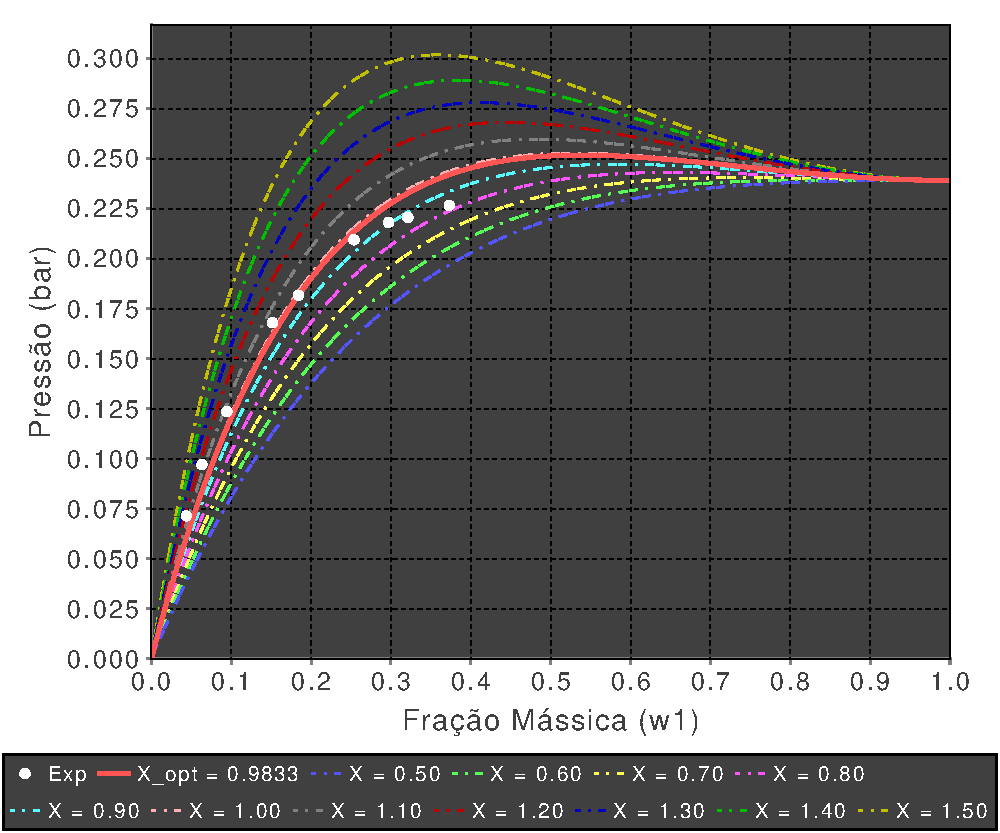
\includegraphics[width=0.8\textwidth]{img/Trab4Abs.pdf}} 
\caption{Curvas $P-w_1$ para diferentes valores de $\chi$ com valor otimizado
(minimizando a diferença dos erros absolutos)}
\label{fig:trab4abs}
\end{figure}



\begin{table}[htb]
\centering
\renewcommand{\arraystretch}{1.1}
\caption{Resposta da otimização com o erro médio absoluto como função
objetivo}
\begin{tabular}{S[table-format=1.4,round-mode=places,round-precision=4]
S[table-format=1.4,round-mode=places,round-precision=4]
S[table-format=1.4,round-mode=places,round-precision=4]
S[table-format=2.0,round-mode=places,round-precision=0]
S[table-format=1.4,round-mode=places,round-precision=4]}
\toprule
\multirow{2}{*}{$\chi_{opt}$}& {Erro Abs.} & {Erro Rel.} & {N$^\circ$
iterações} & {Valor da}\\
& {Médio} & {Médio ($\%)$} & {realizadas} & {$f_{obj}$}\\
\midrule
0.9833&0.0089&6.4287&38&0.0089\\
\bottomrule
\end{tabular}
\label{tab:Opt2T1}
\end{table}

\subsubsection{Otimização - Erro Relativo}
A função objetivo utilizada para o erro relativo é mostrada na
\autoref{eq:fobjrel}. A minimização é feita alterando o valor de $\chi$ e a
função é um somatório, para todos os pontos avaliados (NP), da diferença, em módulo, da pressão 
experimental ($P^{exp}$) e da pressão calculada via o modelo ($P^{calc}$),
divindido tal pela pressão experimental.

\begin{equation}\label{eq:fobjrel}
min_\chi f_{obj} = \sum_i^{NP}\frac{1}{NP}\left| \frac{P_i^{exp} -
P_i^{calc}}{P_i^{exp}} \right|
\end{equation}


A \autoref{fig:trab4rel} mostra o comportamento da função para diferentes
valores de $\chi$, bem como a curva otimizada para o erro relativo. Observa-se
que, desta vez, a curva otimizada passa exatamente sobre o quarto ponto
experimental. Já a \autoref{tab:Opt3T1} apresenta os valores alcançados pela
otimização e o valor de $\chi$ ótimo ($\chi_{opt}$). Os valores relativos a cada
ponto experimental estão presente no Apêndice B.


\begin{figure}[htb]
\centering
{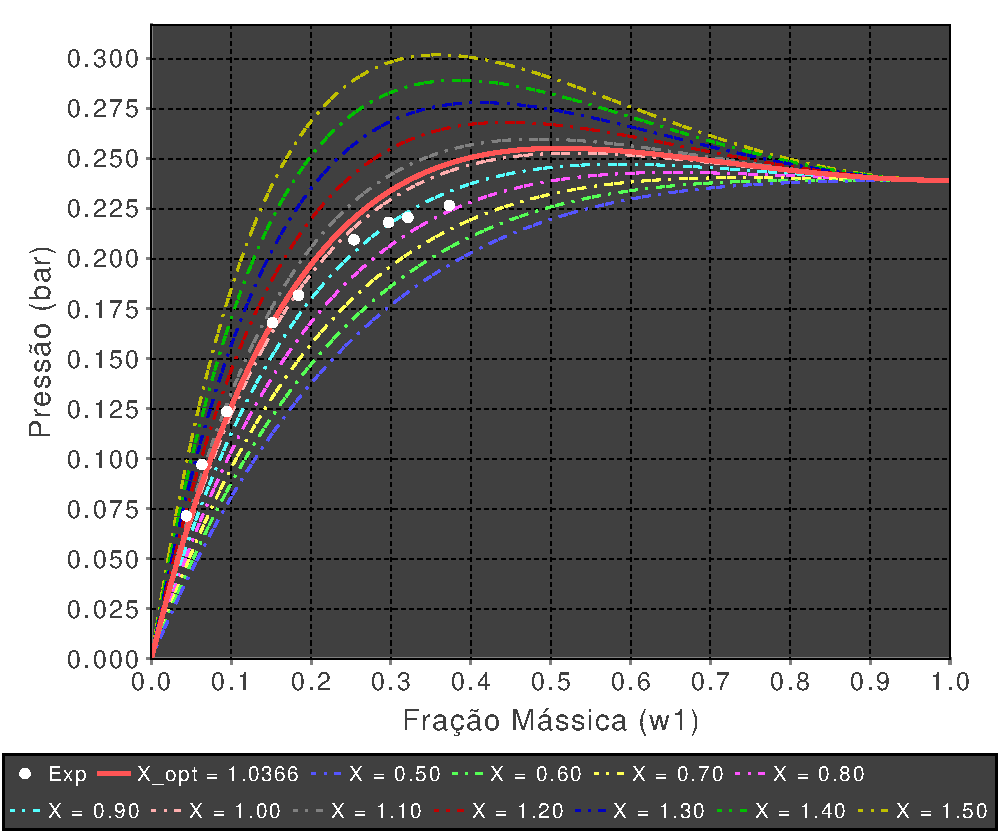
\includegraphics[width=0.8\textwidth]{img/Trab4Rel.pdf}} 
\caption{Curvas $P-w_1$ para diferentes valores de $\chi$ com valor otimizado
(minimizando a diferença  dos erros relativos)}
\label{fig:trab4rel}
\end{figure}

\begin{table}[htb]
\centering
\renewcommand{\arraystretch}{1.1}
\caption{Resposta da otimização com o erro médio relativo como função
objetivo}
\begin{tabular}{S[table-format=1.4,round-mode=places,round-precision=4]
S[table-format=1.4,round-mode=places,round-precision=4]
S[table-format=1.4,round-mode=places,round-precision=4]
S[table-format=2.0,round-mode=places,round-precision=0]
S[table-format=1.4,round-mode=places,round-precision=4]}
\toprule
\multirow{2}{*}{$\chi_{opt}$}& {Erro Abs.} & {Erro Rel.} & {N$^\circ$
iterações} & {Valor da}\\
& {Médio} & {Médio ($\%)$} & {realizadas} & {$f_{obj}$}\\
\midrule
1.0366&0.0103&6.2777&44&0.0628\\
\bottomrule
\end{tabular}
\label{tab:Opt3T1}
\end{table}

A diferença entre os resultados é explicada pelo fato da função objetivo erro
relativo possuir a divisão pela pressão experimental em cada ponto. Assim, nesta
função objetivo, quanto mais próximo de zero é a pressão, maior será o erro gerado 
e, consequentemente, maior o impacto do mesmo no somatório. Assim, é
compreensível que esta otimização posicione o ótimo mais a esquerda do que a anterior de modo a “compensar” 
essa divisão.



\section{Conclusões}
Este trabalho visou o estudo da predição e construção de um diagrama de
equílibrio líquido-vapor para uma mistura de um solvente (benzeno) com um polímero
(poliisobutileno - PIB). Para tal, foi utilizada a Lei de Raoult Modificada, a
qual fez o uso da equação de Flory-Huggins como modelo para o coeficiente de
atividade.

Inicialmente, foram arbitrados valores para o coeficiente de interação de
Flory-Huggins ($\chi$) com o intuito de avaliar a influência deste na predição
do equilíbrio. Em seguida, esse mesmo parâmetro foi estimado através da
minimização da função erro médio (absoluto e relativo), com o objetivo de achar
seu valor otimizado, ou seja, aquele que melhor se ajusta aos dados
experimentais. Nesse intuito, utilizou-se a função \emph{simplex Nelder-Mead},
inicializada nos dois valores menores valores avaliados de $\chi$.

As duas otimizações realizadas alcançaram valores ótimos distintos para o
parâmetro $\chi$. Isso se deve ao fato de que a função objetivo erro médio
relativo considera a pressão experimental de cada ponto. Cada ponto
experimental apresenta valores pequenos (inferiores a $1,0$), o que leva a
acréscimos cada vez maiores quando tais pressões tendem a zero. Já a função
objetivo erro médio absoluto, que não apresenta a divisão pelo valor
experimental, busca uma resposta de fato média para a resolução do problema
(comprovado pelo fato da função cruzar a curva experimental na
mediana).

A partir dos resultados apresentados para o parâmetro de interação de
Flory-Huggins, que assumiu valores acima de $0,50$, pode-se concluir que o
sistema estudado apresenta desvios negativos com relação à idealidade, ou seja,
existem forças atrativas entre as moléculas de solvente e as cadeias poliméricas.

 

